%% draft_sections_4_6.tex — NAACL 2027 SRW fragment (Sections 4--6 only)
%% \input this file into paper/srw.tex in place of the three % TODO blocks.
%% Figure labels fig:pipeline / fig:al-scaling are placeholders pending the
%% final figure files (blueprint: Fig 1 = pipeline+data flow, Fig 2 = AL
%% scaling curve or label-provenance distribution).

\section{Methodology}
\label{sec:method}

\subsection{System overview}
\label{sec:method:system}

Our deployed system is a two-channel ensemble over Chinese review text
(Figure~\ref{fig:pipeline}). The \emph{student} channel is a
\emph{hfl/chinese-macbert-base} classifier \citep{cui2020macbert}; the
\emph{judge} channel is a small MLP head on frozen
MegatronBERT-1.3B features. Both channels emit class-probability
vectors $P_s$ and $P_j$, blended with fixed weights $1{:}2$:
\begin{equation}
  \mathrm{dep} \;=\; \tfrac{1}{3}\,P_s \;+\; \tfrac{2}{3}\,P_j .
  \label{eq:dep}
\end{equation}
For the three-class task, a \emph{neutral specialist} refines $\mathrm{dep}$.
Two estimators of $P(\mathrm{neu})$---a frozen-feature MLP head and a
corpus-trained neutral detector---are mixed as
$p_n = 0.6\,P_{\mathrm{neu}}^{\mathrm{head}} +
0.4\,P_{\mathrm{neu}}^{\mathrm{corpus}}$. Writing $r_{+}, r_{-}$ for the
positive/negative masses of $\mathrm{dep}$ renormalized to sum to one, the
specialist distribution and final blend are
\begin{equation}
  \begin{aligned}
    \mathrm{spec} &= \big[(1-p_n)\,r_{+},\; p_n,\; (1-p_n)\,r_{-}\big],\\
    \mathrm{final} &= \frac{\mathrm{dep} + 0.5\,\mathrm{spec}}{1.5}.
  \end{aligned}
  \label{eq:spec}
\end{equation}
A post-hoc temperature $T{=}0.37$ is applied for calibration; it is
argmax-invariant and therefore does not affect accuracy or macro-F1. For
ultra-short slang-only inputs, a rule-based lexicon guard overrides the
ensemble (it never fires on gold-600). The binary task uses the same
dep-blend without the specialist and a fixed 0.5 decision threshold.

\begin{figure}[t]
\centering
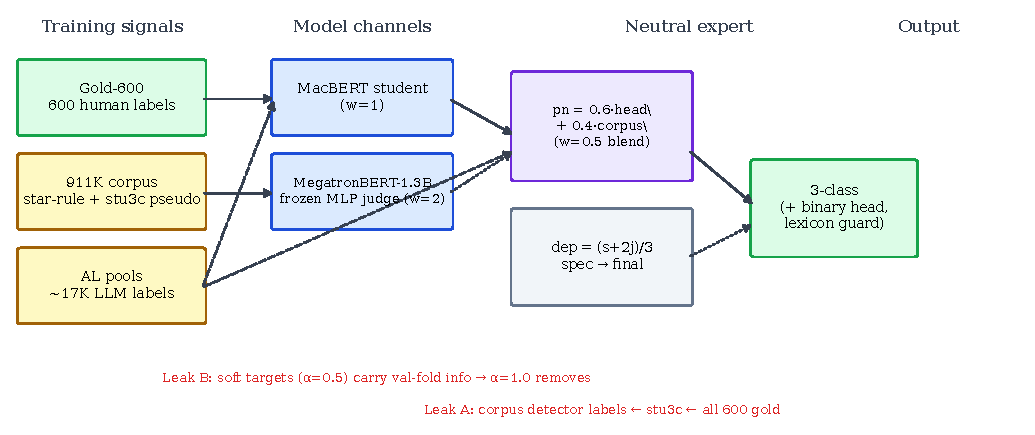
\includegraphics[width=\columnwidth]{fig1_pipeline.pdf}
\caption{Deployed three-class pipeline and its training-signal chain.
Leak~A: the corpus neutral detector's labels descend from stu3c, a
student fit on all 600 gold rows, so its gold predictions carry
whole-set information. Leak~B: distillation soft targets
($\alpha{=}0.5$) are produced by teacher channels whose folds overlap
the student's validation fold. The $\alpha{=}1.0$ ablation removes the
teacher term; the corpus-channel toggle bounds Leak~A.}
\label{fig:pipeline}
\end{figure}

\subsection{Training signal chain}
\label{sec:method:chain}

Labels reach the deployed models through four stages, each of which later
proved relevant to our audit.

\paragraph{Gold seed.} 600 human semantic labels from a single Douban film
page (316 positive / 92 neutral / 192 negative; binary evaluation on the
508 non-neutral rows) provide hard and soft targets for the first students
and judges.

\paragraph{Pseudo-label pools.} Following classical self-training and
pseudo-labeling practice \citep{lee2013pseudo,xie2020selftraining}, a 3-class
student re-scores all 910{,}998 corpus rows under a weak-supervision
framework \citep{ratner2017snorkel}; the confident pool
($\mathrm{conf}{\ge}0.7$, 271{,}905 rows) is sampled under per-class caps into 115K--195K-row
training subsets for full-fit corpus specialists. Binary pools use
$\mathrm{conf}{\ge}0.8$; star-rating-derived label variants serve as
ablations.

\paragraph{Corpus specialists.} Full-fit MacBERT students and frozen-feature
MLP heads are trained on these pseudo-label pools, including the deployed
neutral corpus detector.

\paragraph{Active learning and SFT mixes.} Margin-band
($[0.15,0.70)$) and cross-student disagreement mining select 17{,}000
mutually disjoint corpus rows, which are labeled by LLM teachers
(DeepSeek-V4.1-Flash primary; Qwen3-4B and hybrid variants as comparisons)
in rounds from 1K to 17K labels. A per-fold SFT student is then trained on
gold$+$AL labels and fused with the deployed ensemble at weight $w_{\mathrm{SFT}}$
selected by 5-fold cross-validation.

\subsection{Audit methodology}
\label{sec:audit}

Our contribution is as much the audit as the system. We distinguish
three levels of evaluation independence---\emph{per-row fold
isolation}, \emph{upstream signal isolation}, and \emph{selection
independence}---of which our headline score satisfied only the first,
and even that only up to eight exact-duplicate gold-600 texts that can
cross stratified folds (Appendix~\ref{app:audit} gives the taxonomy).
Two leak
mechanisms violate upstream signal isolation. \textbf{Leak~A}
(transitive pseudo-label): a channel's training labels are outputs of
a model fit on 100\% of the evaluation labels---the chain
gold$\to$stu3c$\to$911K pseudo-labels$\to$corpus detector places gold
information inside the deployed neutral channel at $\approx$13\%
effective weight. \textbf{Leak~B} (second-order teacher): per-fold
soft distillation targets are emitted by teachers whose own folds
overlap the student's validation fold, so at $\alpha{=}0.5$ half the
distillation loss targets contaminated information. Both are invisible
to standard OOF reporting because the CV machinery itself is correct.

Our \emph{leak-isolation protocol} reruns all distilled channels with
$\alpha{=}1.0$ (hard labels only), holding folds, hyperparameters, and
fusion weights fixed, and toggles the corpus channel on/off. A
\emph{row-level cid audit} intersects every evaluation set's comment
IDs with the exact training manifest of each corpus-derived model,
reporting per-model and union overlap plus a near-duplicate check.
A \emph{selection-bias accounting} enumerates the full candidate pool
(26 mixtures, $\approx$73 SFT runs), reports every number as a maximum
over it, and distinguishes cross-fit from oracle selection
\citep{dror2018hitchhiker}. Finally,
all OOD numbers are reported \emph{split by annotation provenance}
(LLM-consensus vs.\ human-adjudicated), and the two LLM passes'
self-consistency is measured on adjudicated rows.

\section{Experimental Setup}
\label{sec:setup}

\paragraph{Evaluation sets.} Table~1 (\S\ref{sec:data}) inventories all
label sources; here we fix the \emph{role} of each set under the audit.
\textbf{gold-600 OOF} was never used for Stage-2 OOD model selection,
but the deployed v3 configuration and its fusion weights \emph{were}
tuned on gold-600 itself, so its OOF estimates are not fully
selection-independent (frozen tuned weights, Leak~A/B bounded by the
$\alpha{=}1.0$ ablation, eight exact-duplicate texts able to cross
folds). \textbf{ood1000} ($n{=}1000$; 800 LLM-consensus + 200
human-adjudicated, the latter labelled with student predictions
visible) is the \emph{development/selection set} for every Stage-2
decision, not a held-out test. \textbf{fresh500} has zero text overlap
with gold/AL pools but $\sim$70\% comment-ID overlap with
corpus-derived training pools, DeepSeek-Flash labels from the same
teacher family as $\approx$16K AL labels, and only the top-2 ood1000
configurations evaluated---a replication check on a partially exposed
distribution. \textbf{lab500} is a superseded, row-level contaminated
pilot used only for annotator-agreement analyses. \textbf{human400}
($n{=}400$) is our identifier-disjoint final test (length-stratified,
single-author blind labels, zero identifier overlap verified post-hoc;
text-level audit: Appendix~\ref{app:human400}).

\paragraph{Metrics and statistics.} We report accuracy and macro-F1 for
both tasks, plus per-class recall to expose neutral-class collapse.
Comparisons use McNemar's exact test, 5{,}000-resample bootstrap confidence
intervals, and Holm correction over the 22-test comparison family
\citep{dror2018hitchhiker}.

\paragraph{Systems compared.} Deployed v3 (uncorrected and $\alpha{=}1.0$
ablations); SFT mixtures at AL scales 1K--17K; TF-IDF and frozen-feature MLP
baselines; Qwen3-4B zero-shot; DeepSeek-V4.1-Flash and V4-Pro zero-shot
teachers.

\paragraph{Implementation.} MacBERT-base student; frozen MegatronBERT-1.3B
judge; 5-fold \texttt{StratifiedKFold} (seed 42, no group constraints)
for gold OOF and seed-0
cross-fit for mixture weights; seeds \{42, 123, 456, 789, 999\}; distillation
$\alpha\in\{0.5,1.0\}$, $\tau{=}2$, 8 epochs. Full hyperparameters are
released with the code and configuration log.

\section{Results and Analysis}
\label{sec:results}

\subsection{Headline correction: what the audit removed}
\label{sec:res-correction}

Table~\ref{tab:main-results} contrasts our previously reported (uncorrected)
headline with the leakage-reduced $\alpha{=}1.0$ rerun. The three-class deployed
89.5\%/85.9\% decomposes cleanly: Leak~B (second-order teacher targets)
accounts for $+5.5$pp accuracy ($89.5\to84.0$ with the corpus channel kept),
and the transitive corpus channel (Leak~A) contributes a further
$+0.7$pp that vanishes when it is removed ($84.0\to83.3$). The
leakage-reduced OOF range is therefore
\textbf{83.3--84.0\% accuracy / 76.3--77.5 macro-F1} for three-class on
the 600 rows (the deduplicated rerun below gives 82.6--83.1\%). The
binary pipeline has no corpus channel, so its entire inflation ($+3.0$pp)
is Leak~B, leaving \textbf{92.9\%/92.4\%} (91.5\%/90.8 deduplicated).
These are leakage-channel ablation estimates, not a fully nested,
selection-independent final-system score: a single seed, frozen
deployed weights tuned on gold-600, $\alpha{=}1.0$ not re-tuned, and
the residual duplicate-text channel disclosed below.
We state plainly that our earlier headline claims were inflated; the
honest numbers are the contribution.

\begin{table}[t]
\centering
\footnotesize
\begin{tabular*}{\columnwidth}{@{\extracolsep{\fill}}lp{3.5cm}cc@{}}
\toprule
Task & Pipeline variant & Acc & Macro-F1 \\
\midrule
\multirow{4}{*}{3-class}
 & deployed, uncorrected ($\alpha{=}0.5$) & 89.5 & 85.9 \\
 & $\alpha{=}1.0$, corpus kept & 84.0 & 77.5 \\
 & $\alpha{=}1.0$, corpus removed & 83.3 & 76.3 \\
 & $\alpha{=}0.5$, corpus removed & 87.5 & 81.3 \\
\midrule
\multirow{2}{*}{binary}
 & deployed, uncorrected ($\alpha{=}0.5$) & 95.9 & 95.6 \\
 & $\alpha{=}1.0$ (no corpus channel) & 92.9 & 92.4 \\
\bottomrule
\end{tabular*}
\caption{Gold-600 out-of-fold results (\%). ``Uncorrected'' rows are the
previously reported deployed scores; $\alpha{=}1.0$ rows remove second-order
teacher leakage (Leak~B). The corpus-channel toggle bounds Leak~A.
Leak~B $\approx{+}5.5$pp (3-class) / ${+}3.0$pp (binary); Leak~A
$\approx{+}0.7$pp.}
\label{tab:main-results}
\end{table}

\paragraph{Duplicate-text leakage.} A further channel affects even the
$\alpha{=}1.0$ estimates: gold-600 has 600 rows but only 592 unique
texts---8 exact-duplicate pairs (Appendix~\ref{app:audit})---and every
OOF script uses stratified $k$-fold without group constraints, so
duplicates can cross folds (expected $\approx$6--7 of 8 pairs),
violating per-fold isolation for these pairs; we estimate the inflation
at $\sim$1--2pp, concentrated in neutral/negative classes. Retraining
the full pipeline on the 592 unique texts with dedup-aligned teachers
moves the $\alpha{=}1.0$
estimates to \textbf{82.6--83.1\%} three-class / 74.8--75.9 macro-F1
and \textbf{91.5\%} / 90.8 binary (from 83.3--84.0 / 76.3--77.5 and
92.9 / 92.4 on the 600 rows); the $\alpha{=}0.5$ variant drops more
(86.5\% vs.\ 89.5\%) since teacher targets also encoded the
duplicates.

\subsection{Out-of-distribution evaluation under selection and provenance}
\label{sec:res-ood}

\paragraph{ood1000 is a development set.} Every Stage-2 decision was made by
reading ood1000 accuracy: AL scale (1K$\to$17K), teacher choice
(DeepSeek/Qwen/hybrid), per-task epochs, seed count and subset, and fusion
weights via cross-validation on ood1000 itself---26 mixture configurations
and $\approx$73 SFT runs in total. Out-of-distribution claims are only as
honest as the selection protocol behind them \citep{baran2023ood}; we
therefore report ood1000 numbers as \emph{development estimates} with an
estimated best-of-$N$ optimism of
$+0.3$--$1.0$pp (3-class) and $+0.2$--$0.7$pp (binary), and McNemar tests
on this set are anti-conservative because it was reused for selection. The
best measured configuration (al17kds mix) reaches 77.1\%/77.4 (3-class)
and 92.3\%/92.1 (binary, $n{=}673$ non-neutral) versus v3's 65.0\%/85.0\%.
On \textbf{fresh500}---a replication check on a partially exposed
distribution (zero text overlap with gold/AL pools, $\sim$70\%
comment-ID overlap with corpus-derived training sets, DeepSeek-Flash
labels from the same teacher family as $\approx$16K AL labels)---the
fixed al17k recipe replicates at 77.0\%/93.7\% versus v3's 58.8\%/86.3\%,
but it measures agreement with teacher conventions as much as
generalization.

\paragraph{Row-level contamination.} Our cid audit shows evaluation texts
entered corpus training sets: 68.7\% of ood1000, 70.2\% of fresh500, and
74.8\% of lab500 rows share a corpus ID with at least one
corpus-trained model, plus 220/107 near-duplicate rows on ood/fresh; the
deployed neutral detector trained on 13.0\% of ood1000 and 13.2\% of
fresh500. AL/SFT pools have \emph{zero} cid overlap, so SFT-mix gains
cannot be explained by row memorization, but every corpus-channel number
carries bounded exposure.

\paragraph{The provenance split is the most consequential finding.}
Table~\ref{tab:ood-results} splits ood1000 by label provenance. Every
system drops 20--32pp on the 200 human-adjudicated rows, which are
disagreement-enriched and intrinsically harder; on this subset the
ranking changes: DeepSeek-V4.1-Flash zero-shot (59.5\%, $n{=}195$)
\emph{exceeds} our best local mixture (56.0\%), while v3 falls to
46.5\%. The two LLM annotation passes agree on only 29.8\% of the 47
adjudicated rows ($\kappa{=}{-}0.18$) versus 100\% on consensus rows by
construction, indicating consensus labels encode a single model's
conventions \citep{schroeder2025humanloop,moller2024parrot}---part of
the mixture's consensus-subset lead is label-convention alignment, not
broad generalization. Binary is more robust: the best mix loses only
8.4pp across provenance (93.7$\to$85.3) versus 26.4pp for three-class.

\begin{table}[t]
\centering\scriptsize
\setlength{\tabcolsep}{2.5pt}
\begin{tabular}{llcccc}
\toprule
Eval rows & $n$ & v3 & al17kds mix & DS-Flash & Qwen3-4B \\
\midrule
ood1000, all (dev) & 1000 & 65.0 & 77.1 & 82.0 & 70.6 \\
\quad LLM-consensus & 800 & 69.6 & 82.4 & 87.5 & 75.1 \\
\quad human-adjudicated & 200 & 46.5 & 56.0 & 59.5 & 52.5 \\
\midrule
fresh500 (DS labels) & 500 & 58.8 & 77.0 & --- & --- \\
\midrule
human400 (blind human) & 400 & 55.8 & 64.8 & --- & 61.5 \\
\bottomrule
\end{tabular}
\caption{3-class accuracy (\%) by evaluation set and label provenance.
ood1000 is a development/selection set; its 200 ``user'' rows were
adjudicated with student predictions visible. DS-Flash parseable $n$:
992 all / 797 consensus / 195 adjudicated. human400 labels are
single-author blind annotations on an identifier-disjoint,
length-stratified sample (text-level audit:
Appendix~\ref{app:human400}); mix uses frozen ood1000-selected weights
(\S\ref{sec:res-human400}).}
\label{tab:ood-results}
\end{table}

\subsection{The identifier-disjoint human test: human400}
\label{sec:res-human400}

human400 is the only evaluation set in this paper with \emph{zero
known identifier overlap} with any training pool and fully human
labels: 400 corpus reviews, length-stratified (160/120/80/40),
sampled with every known training and evaluation pool excluded by
identifier and blind-labelled by a single author (Appendix
\ref{app:annotation}, \ref{app:human400}). Labels: 156~positive / 179~neutral / 65~negative;
single-annotator, so no human--human IAA is available, and the
stratified sample is a benchmark, not a population estimate. A
text-level overlap audit (exact, normalized, near-duplicate) found
zero exact or near-duplicate overlap with the pools of evaluated
systems and only two ultra-short normalized matches in corpus
pseudo-label pools (Appendix~\ref{app:human400}).

On it, deployed v3 reaches 55.8\% three-class accuracy (macro-F1
55.4) and 76.5\% binary accuracy on the 221 non-neutral rows---far
below its dev-set estimates and below its 58.8\% on fresh500's
teacher labels. A star-rating lookup (4--5$\to$positive, 3$\to$neutral,
1--2$\to$negative) achieves \emph{exactly} the same 223/400 correct
(55.75\%): per-rating, only 62.7\% of 5-star and 50.7\% of 4-star
reviews are human-positive---stars encode recommendation intent, not
semantic stance.

The frozen-weight al17k mixture reaches \textbf{64.8\%} three-class
accuracy (macro-F1 63.5), $+9.0$pp over both v3 and the star lookup
(McNemar $p{=}1.3{\times}10^{-3}$ and $7.4{\times}10^{-3}$;
Appendix~\ref{app:human400}). This \emph{reverses} the teacher-alignment
worry: on these identifier-disjoint human labels the AL gains are
genuine generalization. Caveats: accuracy on annotator-flagged
\emph{mixed} reviews drops below v3 (40.0\% vs.\ 53.3\%, $n{=}30$);
binary ($n{=}221$) v3 reaches 76.5\%, below the rating rule (83.7\%),
which the frozen mixture matches (83.7\%, macro-F1 81.3 vs.\ 77.9;
McNemar $p{=}0.02$).

\subsection{Ablations and diagnostics}
\label{sec:res-ablations}

Appendix~\ref{app:ablations} collects the statistical diagnostics.
Adjacent AL scales are within noise (al17k vs.\ al14k: McNemar
$p{=}0.064$), so our honest claim is ``17K is at least as good as
14K''; the v2$\to$v3 specialist gain is positive but non-significant
($\Delta$macro-F1 $+1.6$pp; bootstrap 95\% CI $[-0.4,+3.8]$pp). The
OOD drop is \emph{not} a short-text artifact (v3 flat across ood1000
length buckets; neutral recall collapses 51.1$\to$33.3\%).
Inter-annotator agreement is $\kappa{=}0.568$ against a \emph{blended}
human/LLM reference only.

\subsection{Negative results and what would change our conclusions}
\label{sec:res-negative}

Over twenty variants were rejected (Appendix~\ref{app:negative}); the
audit-relevant ones---LoRA underperformance, synthetic-data poisoning,
flywheel degeneration, a failed meta-learner---are direct evidence
that headline selection operated on
ood1000. Three outcomes would further change our conclusions: a
fold-isolated corpus detector, fusion weights re-tuned on clean
channels, and a second annotator on human400; until then, the
deduplicated leakage-reduced OOF estimates (82.6--83.1\% three-class,
91.5\% binary) are the numbers we stand behind.
